\chapter{基于质量表的核子相互作用\label{chapmassN}}
在微观的量子的世界中,我们已经很难直接的观测到具体的物理过程,而只能通过观测这个过程的初态和末态的特征(能级能量、宇称等),以及这个过程的产物($\gamma$射线、X射线、电子等)的特征,来间接的了解这个物理过程。原子核作为一个由两种相互作用的费米子构成的微观量子多体系统,我们通常是通过测量核反应的产物($\gamma$射线、质子、中子等)的特征(时间关联、能量、动量、角分布等)来了解原子核结构和核力的性质等。而根据质能关系,原子核基态的质量可以对应于这个体系的能级能量,即有可能是某个物理过程的初态或末态的能级能量,我们也就有可能通过原子核基态的质量研究关于原子核的结构以及核力等方面信息。

原子核的结合能$B(Z,N)$可以表达为对应的原子核质量$M(Z,N)$与自由质子质量 $m_p=938.272$ MeV 和自由中子质量 $m_n=939.565$ MeV 的关系:
\begin{equation}
B(Z,N)=Zm_p+Nm_n-M(Z,N)
\end{equation}
其中$Z$和$N$分别为为这个原子核的质子数和中子数,由于自由质子质量和自由中子质量是已知的常量,所以原子核的结合能与质量是一一对应的,所以可以看做是等价的关系,并且原子核结合能可以好的对应于原子核体系的系统能级能量,所以下面的讨论都使用原子核的结合能来代表对应的原子核体系的能级。

以最简单的情况,即将相邻的两个中子数相差1的原子核的结合能做差为例进行讨论:
\begin{equation*}
S_n(Z,N)=B(Z,N)-B(Z,N-1)
\end{equation*}
这个公式即单中子分离能的表达式,表示从原子核$(Z,N)$中分离出最外层的一个中子所需要的能量,同时这个公式也可以对应于这样的一个过程:将一个处于基态的原子核$(Z,N)$,给予其一个足够的能量$S_0$,使其刚好能够剥离出一个动能为0的自由的中子,并且此时其剩余的核心$(Z,N-1)$处于一个$\Delta(Z,N-1)$能级的激发态,在这个激发态中我们认为核心$(Z,N-1)$的每个核子与在$(Z,N)$核的基态中的状态是完全相同的,而由于原子核是一个自组织的系统,为了达到系统的最低能量状态,其剩余的核心$(Z,N-1)$原子核结构及其能级会发生变化,释放出$S_\delta$的能量,达到$(Z,N-1)$核的基态2,可以看出$S_n(Z,N)=S_0(Z,N)+S_\Delta(Z,N-1)$,如图\ref{fig_Sn}所示。
\begin{figure}[H]
\centering
\subfigure[]{
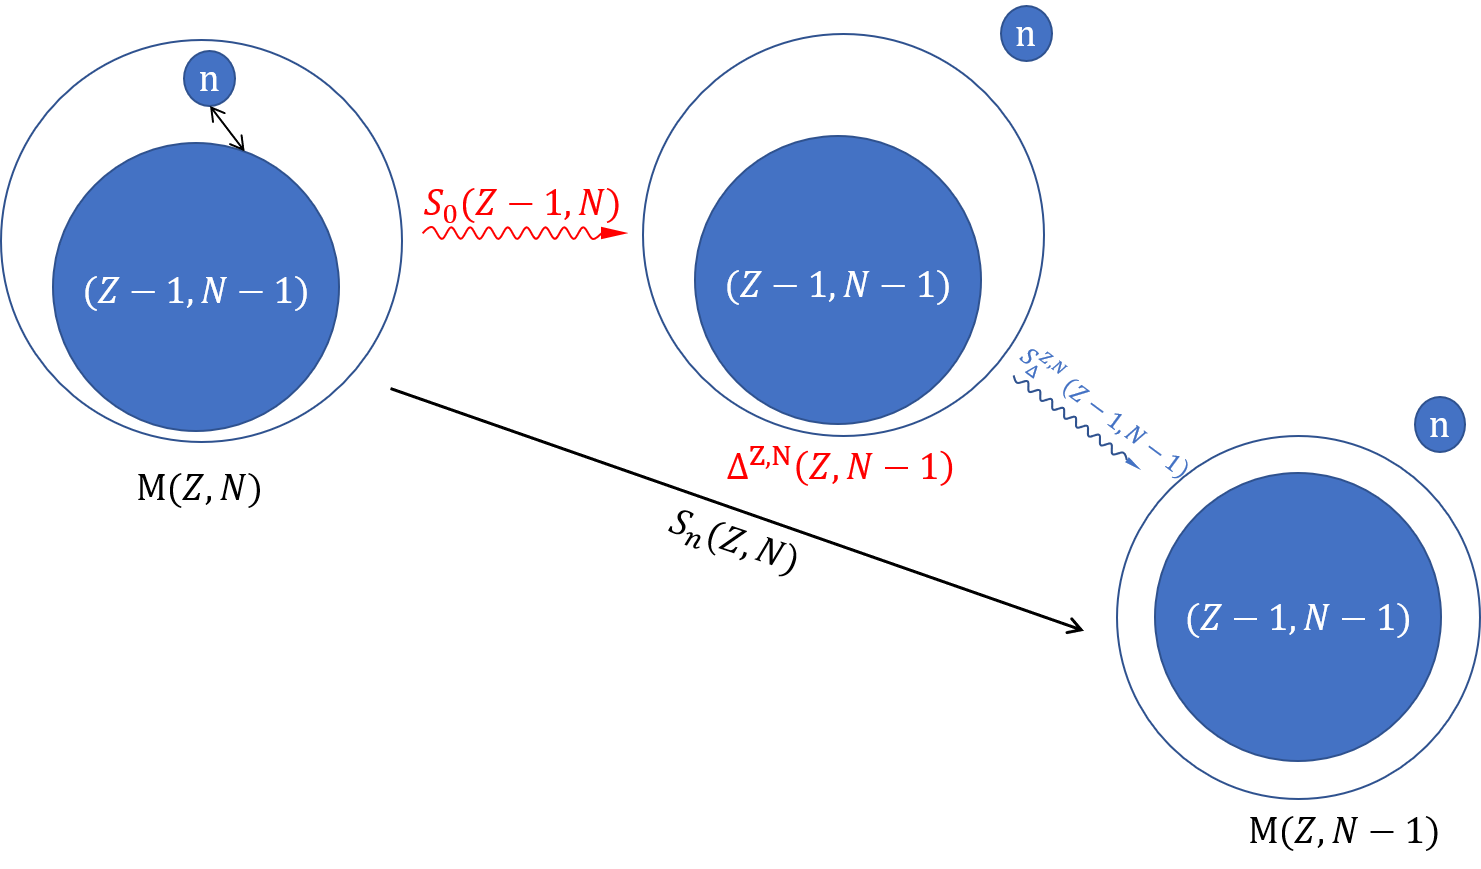
\includegraphics[width=0.5\textwidth]{figure/Sn1.png}}
\quad
\centering
\subfigure[]{
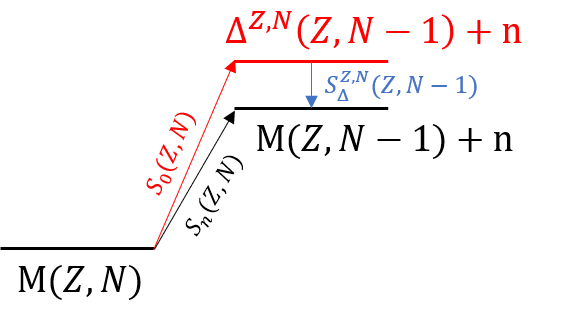
\includegraphics[width=0.4\textwidth]{figure/Sn2.png}}
\caption{单中子分离能$S_n(Z,N)$的物理图像.\label{fig_Sn}}
\end{figure}
需要注意的是这个$\Delta(Z,N-1)$能级是一个我们假想的能级,可能在$(Z,N-1)$核中并不存在这样的一个能级。之所以构想出这样一个复杂的过程,是因为$S_0$可以看做是原子核$(Z,N)$的最外层的中子与这个原子核其余的所有核子的相互作用的总和,如果可以得到这个量,我们就可以利用原子核基态质量来研究核结构与核力的性质。但是,由于原子核$(Z,N-1)$的$\Delta$能级是未知的或不可测量的,所以我们并不能通过$S_n(Z,N)$得到$S_0$,通常我们的做法是如果在移除这个核子后剩余核$(Z,N-1)$相较于原来的核$(Z,N)$没有发生核结构(核子配对、幻数壳层等)的变化,就认为$S_\Delta$相较于$S_n(Z,N)$是非常小的,可以忽略,使得$S_n(Z,N)\approx S_0(Z,N)$,即将$S_n(Z,N)$近似为原子核$(Z,N)$的最外层的中子与这个原子核其余的所有核子的相互作用的总和。所以我们通过原子核基态质量得到的核子相互作用只是真实核力的近似。

提取原子核的最外层的$i$个质子和$j$个中子之间的质子中子相互作用的一般表达式为:
\begin{equation}
\begin{array}{rcl}
V_{ipjn}(Z,N)&=&B(Z,N)-B(Z,N-1)-B(Z-1,N)+B(Z-1,N-1)\\
&=&S_n(Z,N)-S_n(Z-1,n)\\
&=&S_p(Z,N)-S_p(Z,N-1)
\end{array}
\end{equation}
以最简单的原子核的最外层的最后一个质子和最后一个中子之间的质子中子相互作用$V_{1p1n}(Z,N)$为例,如果忽略这几个核的核结构的变化,那么这个公式对应的物理图像应该如图\ref{fig_V1p1n1}所示
\begin{figure}[H]
\centering
\subfigure[]{
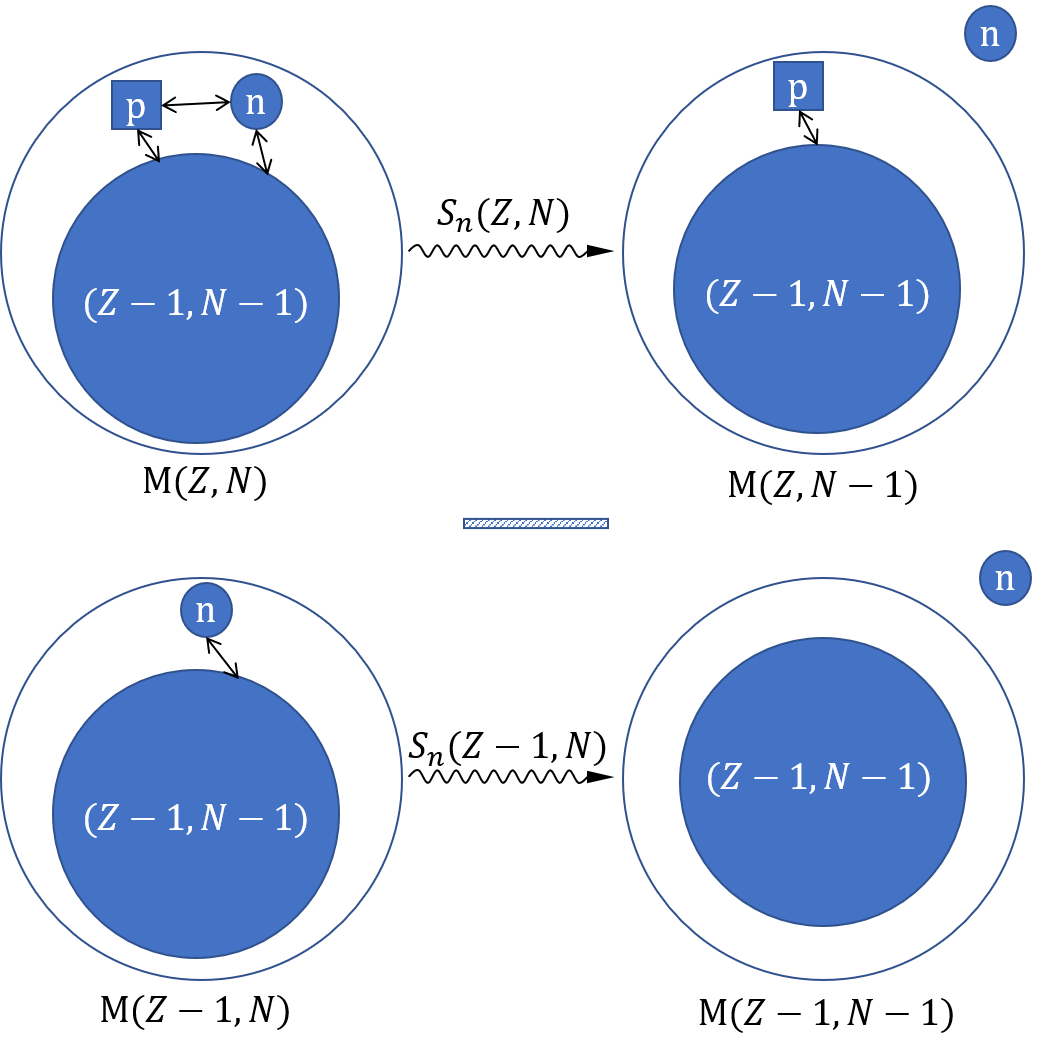
\includegraphics[width=0.5\textwidth]{figure/V1p1n1.png}}
\quad
\centering
\subfigure[]{
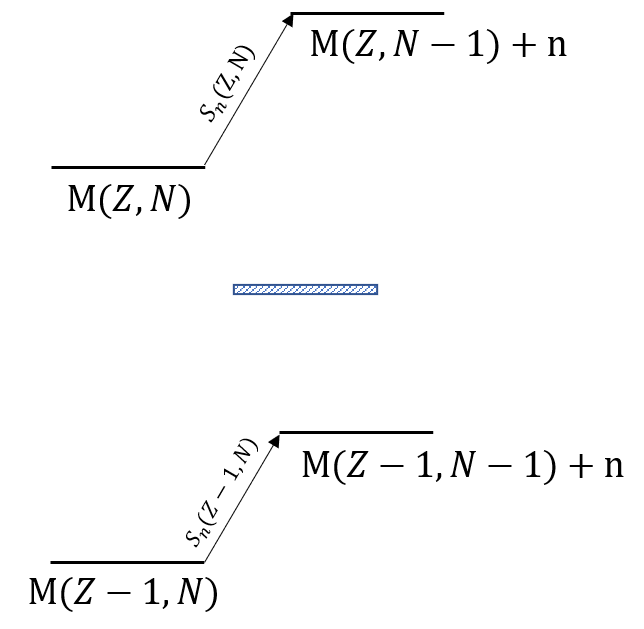
\includegraphics[width=0.4\textwidth]{figure/V1p1n2.png}}
\caption{$V_{1p1n}(Z,N)$的物理图像.\label{fig_V1p1n1}}
\end{figure}

\begin{figure}[H]
\centering
\subfigure[]{
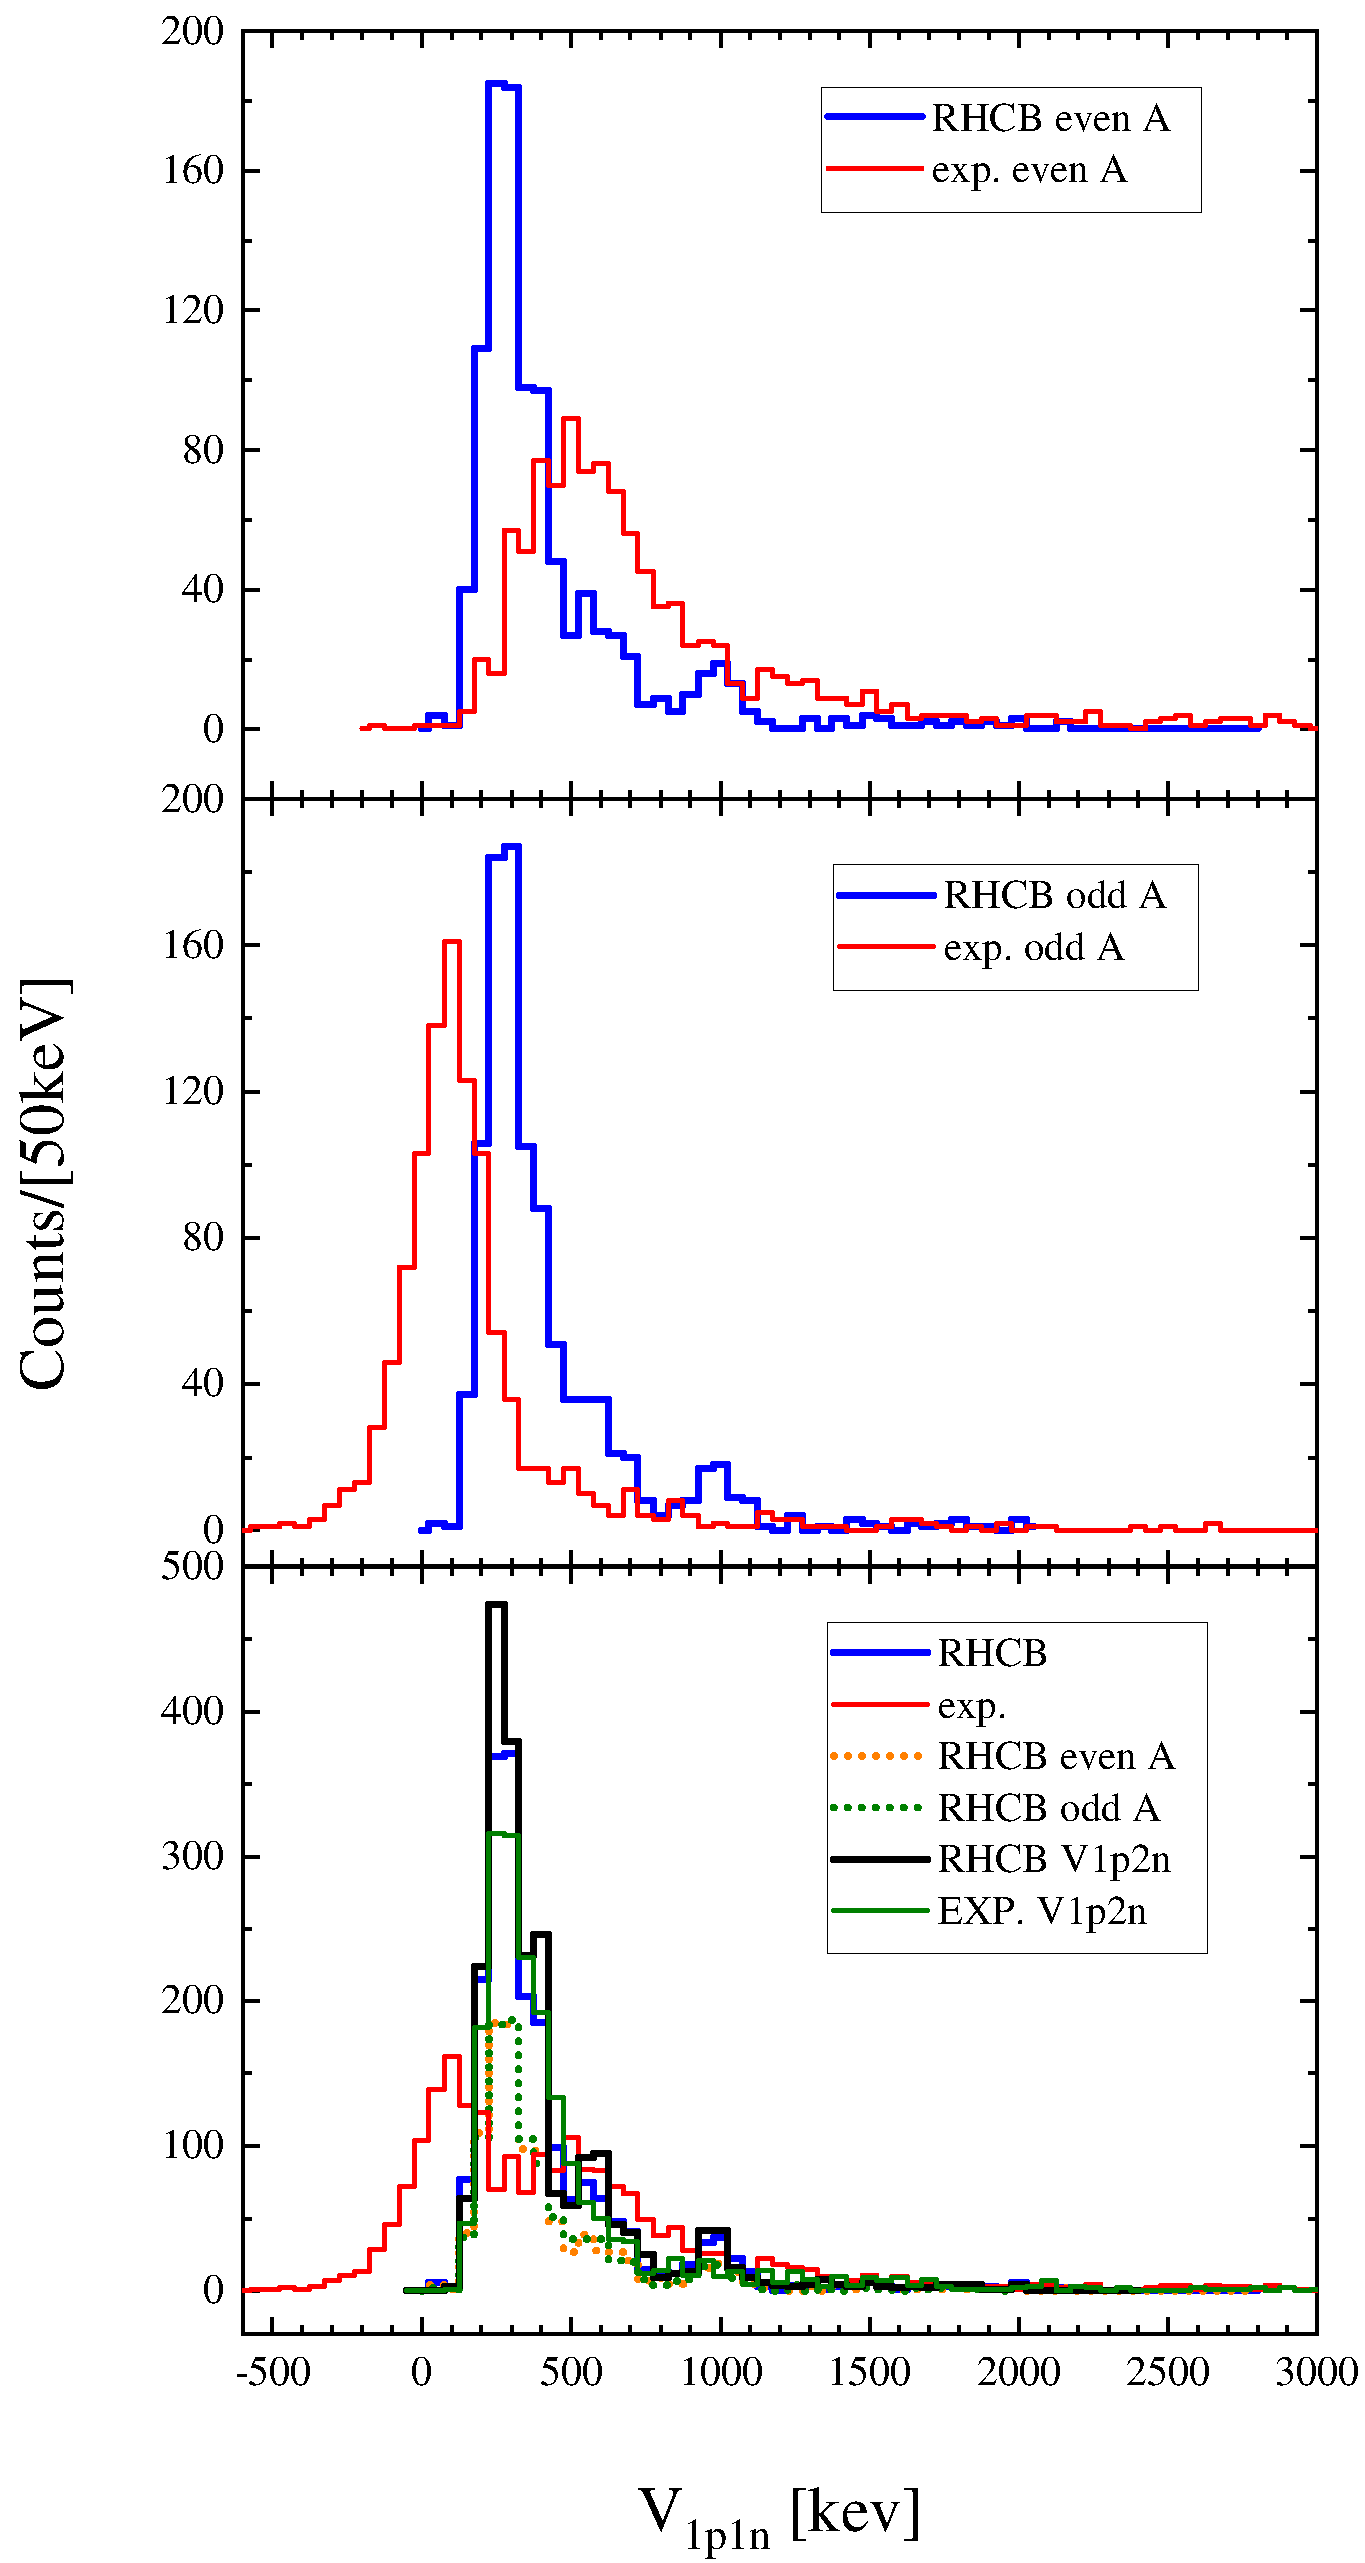
\includegraphics[width=0.4\textwidth]{figure/RHCBV1p1n2.pdf}}
\quad
\centering
\subfigure[]{
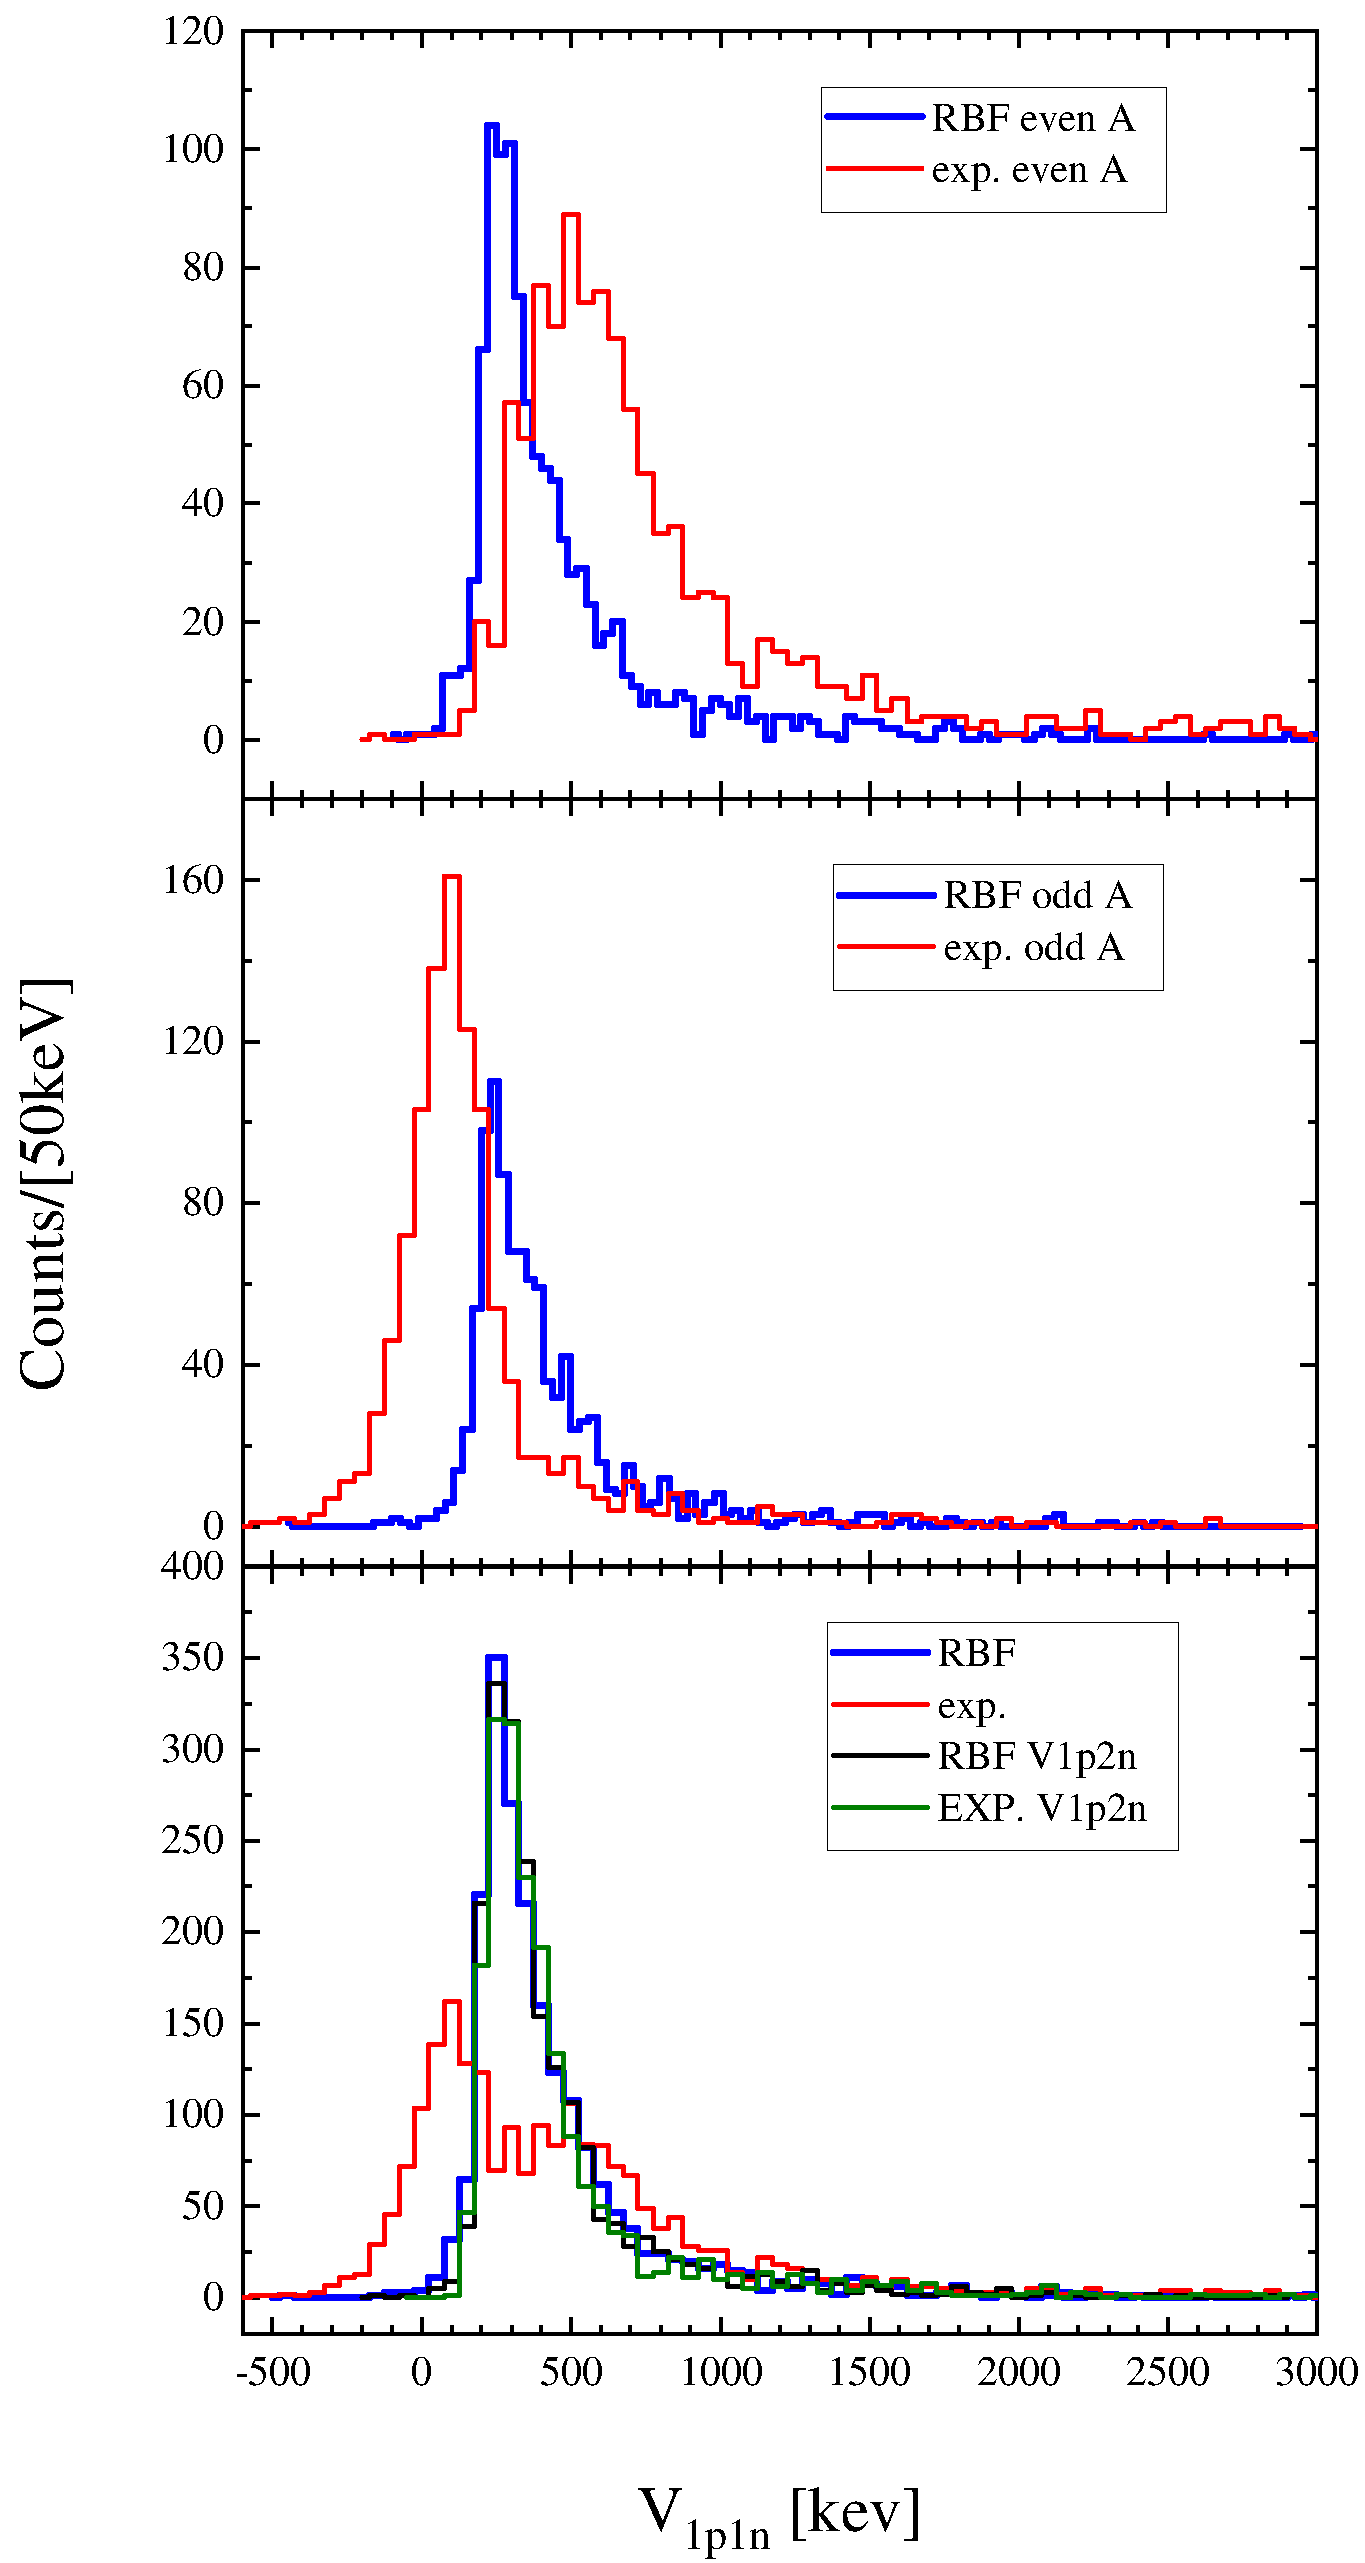
\includegraphics[width=0.4\textwidth]{figure/RBFV1p1n.pdf}}
\centering
\subfigure[]{
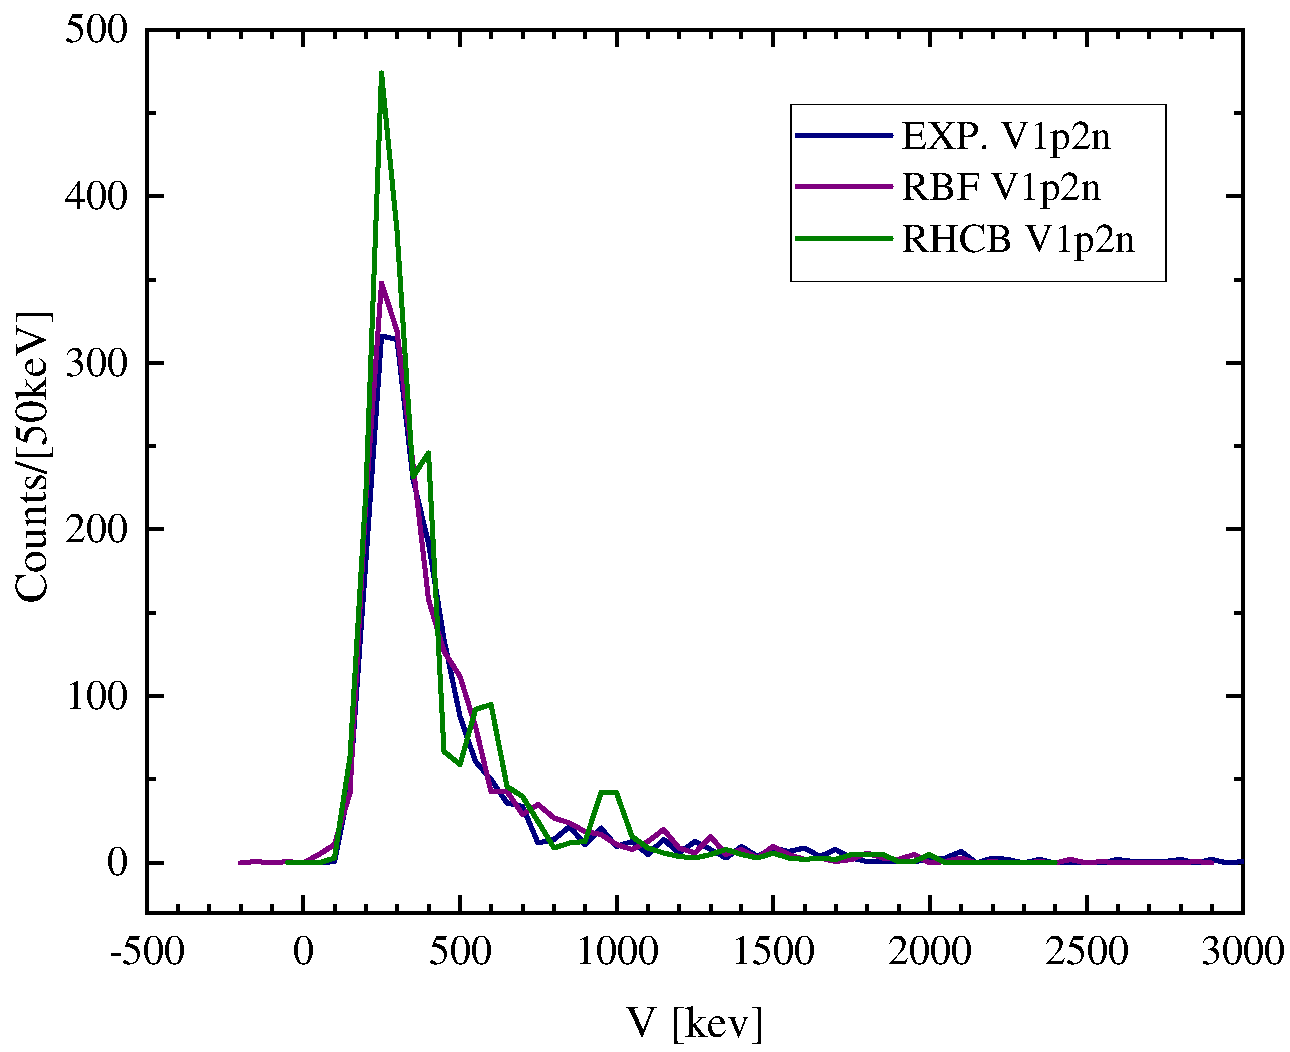
\includegraphics[width=0.7\textwidth]{figure/V1p2npair2.pdf}}
\quad
\caption{$V_{1p1n}(Z,N)$与$V_{1p2n}(Z,N)$.\label{fig_V1p1n1}}
\end{figure}